\hypertarget{a-questuxe3o-do-caruxe1ter-nacional-na-arte-e-na-cruxedtica-da-cidade}{%
\section{A questão do caráter nacional na arte e na crítica da
cidade}\label{a-questuxe3o-do-caruxe1ter-nacional-na-arte-e-na-cruxedtica-da-cidade}}

Na crítica de arte brasileira durante ao menos o meio século que se
estende de 1880 a 1940, a questão do caráter nacional ganha espaço
privilegiado: é nesse contexto que se inserem os discursos e as
temáticas de personagens nacionais, nas artes plásticas, e o movimento
neocolonial em arquitetura. É também ao final desse período que o
Movimento moderno busca afirmar-se como legítimo sucessor nacional dos
estilos tradicionais. A prática e a crítica das artes visuais seguem
nesse período, com alguns anos de descompasso, os precursores
literários, ora inspirando-se nos seus temas explícitos --- como o
indianismo ou o nativismo ---, ora repercutindo o estado da ideologia
nacionalista.

A cultura literária brasileira do Romantismo, por sua vez, promove uma
imagem bastante elogiosa de si mesma. As revisões historiográficas
gabam-se da existência de uma literatura com feição nacional própria que
remonta, ao menos, a meados do século XVIII. Tal interpretação é vigente
ao menos desde Gonçalves de Magalhães, para quem Basílio da Gama ``canta
como Homero, sem deixar de ser brasileiro''
\autocite*[p.~47]{magalhaes:1834resume}, inserindo-se numa compreensão
totalizante da história da literatura como história da civilização
\autocite[p.~140]{botelho:2011pequena23}. Atestada entre os primeiros
etnógrafos portugueses, a exemplo de Teófilo Braga
\autocite*{braga:1870historia}, essa historicização total coaduna com a
``historiografia oficial'' do círculo do IHGB para moldar a narrativa de
uma gradual, inevitável e lisonjeira caracterização da (alta) cultura
nacional brasileira. O determinismo geográfico e racial assim formulado,
e ainda presente na síntese histórica tardia de Ronald de Carvalho, de
1919, pode até fazer a emancipação cultural, situada na segunda metade
do Setecentos, prenunciar a independência política
\autocite[p.~47]{carvalho:1937pequena}. Mesmo a interpretação mais
moderada de Sylvio Roméro e José Veríssimo
\autocite[p.~143]{botelho:2011pequena23} vê na literatura nacional um
relato de contínuo progresso desde o início do romantismo.

Os artistas e arquitetos de maior projeção na capital estão, até os
últimos anos do Império, essencialmente interessados na consolidação do
ensino artístico e da inserção dos profissionais no mercado e na
formulação de políticas urbanas, como indicam os artigos de Araújo
Porto-Alegre na revista \emph{Guanabara} e os debates do arquiteto e
professor da academia Francisco Joaquim Bethencourt da Silva
(1831--1911) na imprensa carioca. Cabe à crítica de arte diletante, que
toma forma nesse período principalmente sob a pena do jornalista Luiz
Gonzaga Duque Estrada (1863--1911), adotar um olhar combativo a respeito
da ``evolução'' da cultura brasileira e instar a prática da pintura num
rumo convergente com o da literatura romântica. Na década de 1880, temas
pictóricos tomados à literatura indianista vêm a ser usados na pintura
acadêmica brasileira. Ao final da mesma década, paradoxalmente, o jovem
crítico de arte Gonzaga Duque lamenta o desaparecimento do caráter
nacional na arte. No livro síntese do seu pensamento de juventude,
\emph{A Arte Brasileira} (1888), ele traça um panorama pessimista da
arte nacional:

\begin{quote}
O romance, a poesia e a história do país nenhuma influência tiveram
nessas obras que permaneceram invioláveis ao pálido alvorecer do
pensamento nacional. {[}\ldots{]} Conclui-se, pois, que a esta arte
faltam --- feição nativa e originalidade, primordiais qualidades para a
fundação de uma escola.

{[}\ldots{]} a feição que caracteriza a nossa arte é o cosmopolitismo, e
um país para ter uma escola precisa, antes de tudo, de uma arte
nacional. \autocite[p.~258--259]{gonzagaduque:1995arte}
\end{quote}

No entanto, Gonzaga Duque tampouco se empolgava com a arte dos períodos
anteriores. Mesmo a arquitetura monumental do Brasil colônia, que
cativou autores subsequentes, era para ele ``uma flagrante prova do mau
gosto e da falta de inteligência''
\autocite[p.~74]{gonzagaduque:1995arte}. Mal e mal concedia aos pintores
do século XVIII, como Manoel da Cunha (1737--1809), uma aura de aplicada
sinceridade \autocite[ p.~81]{gonzagaduque:1995arte}.

Ao contrário do que pregavam os românticos europeus, portanto, Gonzaga
Duque não sugeria a produção de uma arte nacional baseada nas
realizações das épocas mais antigas da história do próprio país. O
caráter nacional adviria do amadurecimento daquela mesma arte acadêmica
do seu tempo. Nesse aspecto, mesmo um jovem e promissor artista como
Rodolfo Amoedo --- a quem Gonzaga Duque encomendou o próprio retrato ---
era censurado pela fraqueza dos seus temas. Assim, na obra de juventude
de Gonzaga Duque, o caráter nacional não era uma expressão estilística,
mas sobretudo a escolha dos temas adequados, sobretudo os indianistas
\autocite[p.~185]{gonzagaduque:1995arte}.

\begin{center}\rule{0.5\linewidth}{0.5pt}\end{center}

Em 1888, um jovem Gonzaga Duque censura o pintor Almeida Júnior
(1850--1899) por não adotar a temática indianista em suas obras.

\begin{center}\rule{0.5\linewidth}{0.5pt}\end{center}

Cenas de gênero ou da vida de pessoas de classes sociais baixas,
frequentemente retratadas com uma linguagem impressionista, ganham
aceitação nos salões de arte já no início da República.

\begin{center}\rule{0.5\linewidth}{0.5pt}\end{center}

Em 1909, no entanto, a sua posição havia se modificado: naquele ano,
Gonzaga Duque elogiava Amoedo por ter superado a fixação indianista,
``vencido pela força assimiladora dum meio superior.''
\autocite[p.~13]{gonzagaduque:1929contemporaneos}: qual fosse, a cultura
pictórica europeia, na forma de nus clássicos e cenas da mitologia
antiga. No último apanhado que fez da arte brasileira, o discurso de
abertura da Exposição Geral de Belas Artes de 1908, no Rio de Janeiro,
Gonzaga Duque resumiu um retrato triunfal da arte nacional. Ele não
julgava mais a arte colonial pelo seu valor estético, mas a considerava
um ``documento histórico'' da maior importância
\autocite[p.~247]{gonzagaduque:1929contemporaneos}. Ao mesmo tempo, a
influência francesa que ele lamentara na sua juventude não era mais
considerada algo que dificultasse a expressão do caráter nacional. Ao
contrário, ela fornecia as indispensáveis perícia técnica e ambiência
cultural a partir das quais o caráter nacional emergiria naturalmente.

A herança colonial de matriz portuguesa e católica tornou-se, então, uma
ancestralidade mítica do caráter nacional vindouro ou contemporâneo.
Origem reverenciada formalmente, mas exercendo influência quase nula nas
concepções vigentes de arte nacional. Gonzaga Duque, proferindo seu
discurso diante dos professores da Escola Nacional de Belas Artes, foi
ponderado na sua definição de caráter nacional:

\begin{quote}
{[}\ldots{]} a arte caracteristica, verdadeiramente brasileira, surgirá
desta natureza admiravel, desta luz de ouro, dessa alma popular feita
com a nostalgia do indio, a infallibilidade animal do africano e a alma
lyrica do portuguez marujo e exul. \autocite[
p.~255]{gonzagaduque:1929contemporaneos}
\end{quote}

\begin{center}\rule{0.5\linewidth}{0.5pt}\end{center}

The occasion was momentous: 1908 marked the centennial of the transfer
of the Portuguese Crown from Lisbon to Rio, thus marking the onset of a
cycle of direct European influence on all aspects of Brazilian culture.
In Gonzaga Duque's speech, Colonial art was no longer judged by its
aesthetic value---either good or bad---, but seen as a ``historical
document'' of utmost importance \autocite[p.
247]{gonzagaduque:1929contemporaneos}. Conversely, French influence was
no longer seen as harming the expression of national character. On the
contrary, it provided the necessary professional expertise and cultural
environment in which national character would gradually emerge.

The colonial heritage, of Portuguese and Catholic extraction, was thus
granted the status of a mythical ancestor of contemporary national
character: one to which ritual deference was owed, but one that exerted
minimal influence on present conceptions of national art. Gonzaga Duque,
speaking before the assembled professors of the Fine Arts School as well
as the President of the Republic, was cautious in his definition of this
character:

His commentaries on the \emph{Salons} of the years 1904--1907 give,
perhaps, a more vivid picture of what he took this ``truly Brazilian''
art to be. Landscape paintings, adroitly portraying the ``admirable
nature'' with its ``golden light'', were particularly favored and
commended. Scenes of daily life drew a good lot of his attention, as
much as the conventional mythological scenes and classical studies.
Indianist subjects were not altogether disparaged, but they had ceased
to be sufficient reason for a painting or sculpture to be commended.
Religious, historical and allegorical works, supposedly the acme of
academic art, were mostly shunned by the nation's most respected art
critic.

\begin{center}\rule{0.5\linewidth}{0.5pt}\end{center}

Tais discursos, via de regra, postulam uma espécie de retórica da perda,
pela qual convenciona-se que a ``arte tradicional do Brasil'' havia sido
extinta por volta de meados do século XIX. Tal extinção é
predominantemente atribuída à chamada Missão artística francesa.
Todavia, sabe-se que a penetração do neoclassicismo e dos conceitos
acadêmicos e ecléticos fora dos grandes centros litorâneos é, na melhor
das hipóteses, lenta e parcial. Mesmo nas cidades importantes, ademais,
a arte acadêmica ensinada e praticada no Rio de Janeiro é pouco
conhecida, predominando a continuidade de oficinas artísticas e
construtores locais, distantes dos paradigmas eruditos e europeizados da
capital.

Por outro lado, cabe ressaltar em defesa dos autores citados que a
própria continuidade nas tradições artísticas coloniais ao longo do
século XIX é, até meados do século passado, mais do que uma prova da sua
persistência, um empecilho à datação precisa dessas manifestações. Outro
ponto a ser levantado com respeito à definição do que constitui ``arte
tradicional do Brasil'' no século XIX é as alterações pelas quais passa
número não desprezível de exemplares coloniais mais ou menos eruditos,
tais como a Capela do Padre Faria, em Ouro Preto, e o Pátio do Colégio,
em São Paulo. As restaurações destrutivas empreendidas pelo Serviço do
Patrimônio Histórico e Artístico Nacional em meados do século XX, como
apontado por diversos pesquisadores recentes, testemunham uma certa
visão modernista madura, por assim dizer, acerca do que caracterizaria a
autenticidade da arquitetura tradicional. Isso sem falar no problema
ainda mais espinhoso de obras concluídas na segunda metade do século
XIX, porém seguindo padrões estéticos não acadêmicos, tais como a Igreja
São Francisco de Paula, em Ouro Preto, ou as pinturas murais da Fazenda
Resgate, em Bananal (SP). A absoluta centralidade de Ouro Preto, aliás,
no cânone da arquitetura colonial brasileira a partir de meados do
século XX deve ser contraposta ao efetivo conhecimento que dela teriam
os autores metropolitanos no período imediatamente anterior.

\hypertarget{a-suxedntese-pictuxf3rica-do-final-do-suxe9culo}{%
\section{A síntese pictórica do final do
século}\label{a-suxedntese-pictuxf3rica-do-final-do-suxe9culo}}

O próprio Meirelles, em suas telas da Guerra do Paraguai, acabaria se
afastando do paradigma documental e se aproximando da estética romântica
do sublime, mas nunca chegou a aplicá-la a vistas urbanas, tendo se
concentrado na pintura histórica e alegórica até o final de sua
carreira. Assim como na Capital, foi a atuação dos artistas de origem
estrangeira nas províncias --- no caso, imigrantes e seus descendentes,
em vez de viajantes ---, não comprometidos com as estruturas de poder ou
de ensino estabelecidas, que estimulou o desenvolvimento de abordagens
não documentais na iconografia urbana.

A produção de Nicola Antonio Facchinetti (1824--1900) no Rio de Janeiro,
de Pedro Weingärtner (1853--1929) no Sul do Brasil, e de seu coetâneo
Benedito Calixto em São Paulo sintetiza o percurso da iconografia urbana
brasileira no final do século XIX. Facchinetti, o mais velho dos três, e
chegando já adulto ao Brasil, atuou na continuidade da tradição
romântica da vista sublime, na qual a cidade se curva à escala da
natureza.

Weingärtner, nascido em Porto Alegre, conciliou sua formação nas escolas
acadêmicas da Europa com a temática realista que então competia com o
impressionismo pelo título de vanguarda. Seu registro da fundação de
Nova Veneza (Santa Catarina), intitulado Vida nova (1893, Figura
\ref{fig:weingaertner}), sinaliza uma inflexão nas vistas de cidades
brasileiras. Iniciando sua carreira quanto Meirelles já era
nacionalmente consagrado, ele não sentiu a mesma necessidade de se
acomodar num tipo iconográfico convencional, mas tampouco se aproximou
da estética romântica que valorizava a natureza dominante. Sua
composição ``meticulosamente estudada'' \autocite{carvalho:2008paisagem}
equilibra o povoado incipiente e a natureza como fundo, ressaltando um
episódio humano em primeiro plano. Trata-se de uma abordagem que
subverte tanto a dominância da natureza, cara aos românticos, quanto a
hierarquia do panorama documental, destinada a exaltar as sedes urbanas
do poder político e relegando as personagens do povo a detalhes de
ambientação.

\begin{figure}
\hypertarget{fig:weingaertner}{%
\centering
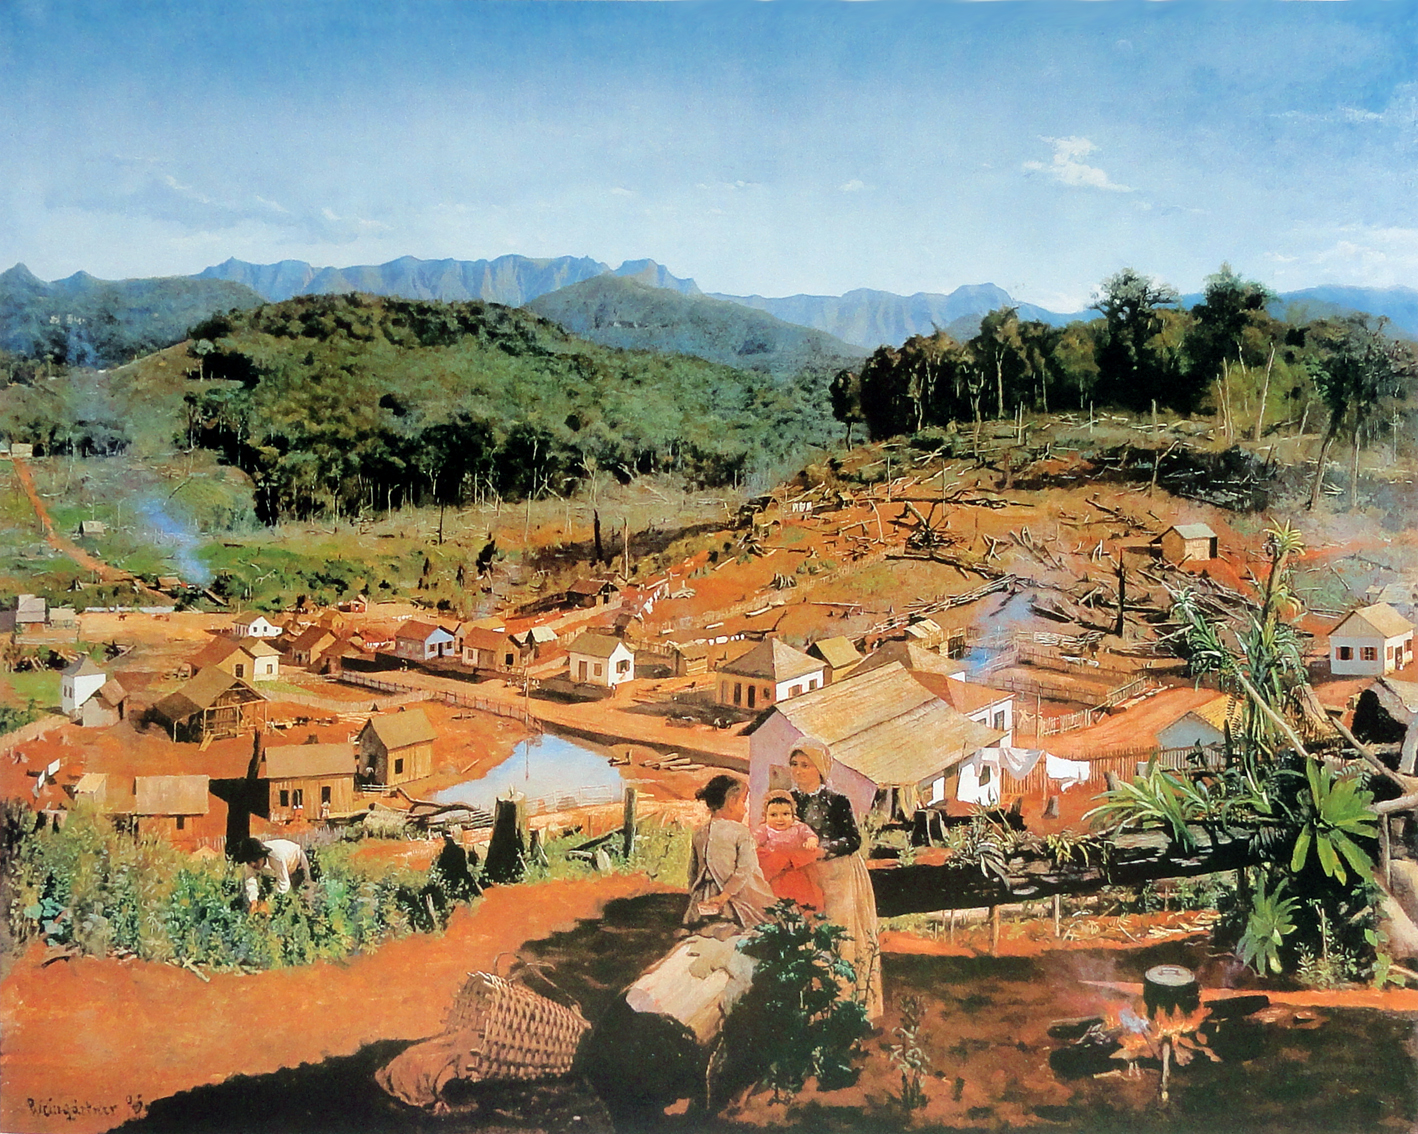
\includegraphics{figures/Pedro_Weingaertner_-_Vida_nova_-_1893.jpeg}
\caption{Pedro Weingärtner (1853--1929). Vida nova,
1893}\label{fig:weingaertner}
}
\end{figure}

Calixto, luso-brasileiro e paulista, destacou-se pelas vistas do litoral
de seu estado, seja no gênero de paisagem ou no da pintura histórica.
Sua canônica representação da Proclamação da República (1893), apesar de
moldada, pela dramatização dos acontecimentos, no triunfalismo
militarista, reatualizou a tipologia documental na tradição de Nicolas
Taunay. A tela (Figura \ref{fig:calixto}) apresenta um espaço urbano
circunscrito, sem ênfase na sua inserção na natureza, servindo como
fundo cênico para um acontecimento histórico. O conjunto da obra de
Calixto transita entre as vistas contemporâneas e o gênero histórico.
Diferentemente do ambiente artístico do início do século XIX, porém, não
há, na produção de Calixto, separação estanque entre os gêneros
pictóricos. Sua atuação remete à prática clássica de inserção de cenas
históricas ou bíblicas em exuberantes paisagens, que, de resto, havia
sido aplicada por Taunay pai no Rio de Janeiro. Por outro lado, a série
de pinturas de Santos e São Vicente, onde residia, quando tomada como
conjunto sobrepõe as múltiplas leituras da vista urbana documental, da
representação de cenas históricas, assim como reminiscências do tema
romântico da natureza pujante.

\begin{figure}
\hypertarget{fig:calixto}{%
\centering
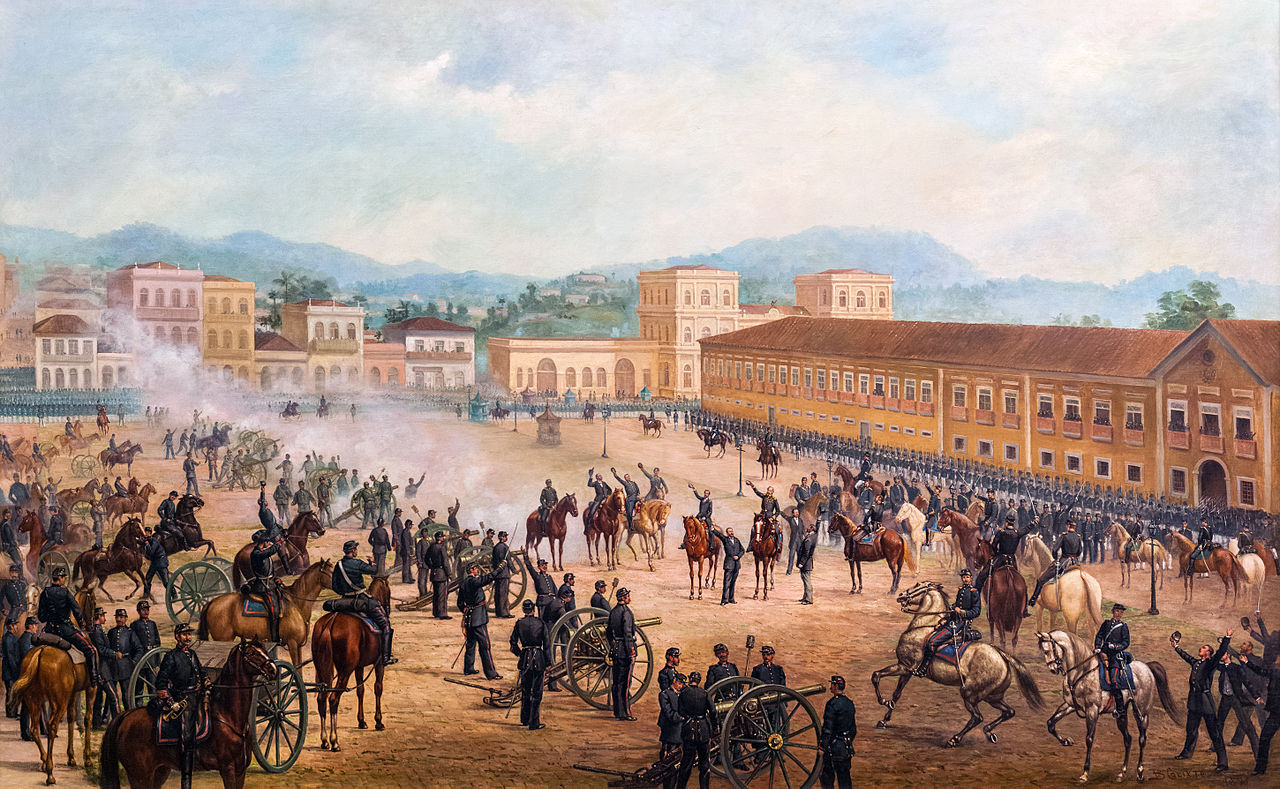
\includegraphics{figures/Proclamacao_da_Republica_by_Benedito_Calixto_1893.jpeg}
\caption{Benedito Calixto (1853--1927). Proclamação da República,
1893}\label{fig:calixto}
}
\end{figure}

A síntese operada nessa combinação de abordagens marca, entretanto, o
canto do cisne da vista urbana enquanto gênero misto de artístico e
documental --- para a geração de José Washington Rodrigues (1891--1957),
a recepção de obras semelhantes terminaria por recair exclusivamente no
seu caráter informativo, ao passo que os modernistas enfatizariam
exclusivamente o aspecto plástico das suas próprias representações de
cidades.
